 \documentclass[12 pt]{book}
\usepackage{amsmath}
\usepackage{amsthm}
\usepackage[paperwidth=5 in,paperheight=5 in,left=9 mm, right=9 mm, top=15 mm, bottom=18.5 mm]{geometry}
\usepackage{graphics}
\usepackage{fontawesome}
\usepackage{enumitem}
\usepackage{marvosym}
\newcommand{\myitem}{\refstepcounter{enumi}\item[$^\star$\theenumi.]}
\newcommand{\mmyitem}{\refstepcounter{enumi}\item[$^{\star \star}$\theenumi.]}
\setcounter{page}{01}

\usepackage[utf8]{inputenc}
\usepackage{xcolor}
\setlength{\arrayrulewidth}{0.1 mm}


%%----HEADER &&& FOOTER----%%

\usepackage{fancyhdr}


\pagestyle{fancy}
\fancyhf{}
\setlength{\headheight}{8 mm}
%\fancyhead[CE,CO]{ \Times\Large{\textbf{\textls*[100]{\textcolor{tomato}{\textit{Illustration}}}}}}

\fancyhead[CE,CO]{\Large{\textbf{\textls*[250]{\textcolor{tomato}{SOLVE ME! \\[-5 mm]{\Large{\textbf{\textls*[5000]{\textcolor{black}{\scalebox{.42}{ROTATION}}}}}}     }}}}}

\fancyfoot[RE,RO]{\large{\textbf{\textls*[10]{\textcolor{tomato}{\Times\textit{Solution~\boldmath$\rightarrow$}}}}}}

\renewcommand{\headrulewidth}{0 mm}
\renewcommand{\footrulewidth}{0 mm}


\DeclareMathOperator{\Ln}{ln}

%%----FONT &&& MATHS_FONT----%%

\usepackage{amssymb}
\usepackage{upgreek,xspace}
\newcommand*{\rom}[1]{\expandafter\@\romannumeral #1}


\usepackage[utopia]{mathdesign}
\renewcommand{\familydefault}{\sfdefault}
\usepackage[scaled=1]{helvet}
\newcommand*\Times{\fontfamily{ptm}\selectfont}

%%%------PACAKAGES------%%%

\usepackage[letterspace=120]{microtype}
\usepackage{enumitem}
\usepackage{multicol}
\usepackage{pgfplots}
\pgfplotsset{width=8cm,compat=1.16}
\usepackage{tikz}
\usepgfplotslibrary{fillbetween}
\usetikzlibrary{quotes,angles,patterns,through,calc}
\usepgflibrary{arrows.meta}
\usetikzlibrary{decorations.pathmorphing}
\usetikzlibrary{decorations.markings}
\usetikzlibrary{arrows.meta,bending}
\usepackage{rotating}
\usepackage{tikz-3dplot}
\usepackage[american voltages, american currents,siunitx]{circuitikz}
\usepackage{circuitikz}
\usetikzlibrary{fit,positioning}
\usetikzlibrary{optics}
\usetikzlibrary{intersections}
\usetikzlibrary{decorations.pathreplacing}
\usepackage{setspace}
\setstretch{1.1}

\usepackage{asymptote}

\usepackage{vwcol}[widths={0.25,0.75}]


\usepackage{color}
\usepackage[autostyle]{csquotes}


\usepackage{xcolor}
\definecolor{Mycolor2}{HTML}{33cccc}
\definecolor{One}{HTML}{336666}
\definecolor{Two}{HTML}{666666}
\definecolor{Three}{HTML}{cc6699}


%  black--brown--black %
\definecolor{Four}{HTML}{000000}
\definecolor{Five}{HTML}{330000}
\definecolor{Six}{HTML}{000000}

\definecolor{Seven}{HTML}{ff6666}
\definecolor{Eight}{HTML}{330066}
\definecolor{Nine}{HTML}{cc3333}
\definecolor{tomato}{HTML}{FF6347}
\definecolor{darkblue}{HTML}{2c3e50}
\definecolor{blackm}{HTML}{363636}
\definecolor{pink}{HTML}{ff6666}


\newcommand{\nm}{\begin{minipage}[c]{0.1\linewidth}
{\Huge{\textcolor{tomato}{\textbf{4. }}}}
\end{minipage}}

\newcommand{\sm}{\begin{minipage}[c]{0.1\linewidth}
{\Huge{\textcolor{tomato}{\textbf{ }}}}
\end{minipage}}

\newcommand{\AxisRotator}[1][rotate=0]{%
    \tikz [x=0.25 cm,y=0.60 cm,line width=.2 ex,-stealth,#1] \draw (0,0) arc (-150:150:1 and 1);%
}

\newcommand{\vl}{{{\textcolor{tomato}{\textbf{\vrule width 2.25 pt{}}}}}}

\newenvironment{question}
{	
	\nm  \vl \,
	\begin{minipage}[l]{0.86\linewidth}
	\begin{itshape}
	\normalsize\Times\textit{}
}
{
	\end{itshape}
	\end{minipage}
}


\newenvironment{options}
{	
	\sm ~
	\begin{minipage}[l]{0.86\linewidth}
	\begin{multicols}{2}
	\begin{enumerate}[label={(\roman*)}, itemsep=4 mm]
	\normalsize{}
}
{
	\end{enumerate}
	\end{multicols}
	\end{minipage}
}


\newenvironment{v-options}
{	
	\sm ~
	\begin{minipage}[l]{0.86\linewidth}
	\begin{enumerate}[label={(\roman*)}, itemsep=4 mm]
	\normalsize{}
}
{
	\end{enumerate}
	\end{minipage}
}



\newenvironment{definition}
{
	\begin{center}
	\begin{itshape}
	\normalsize\Times\textit{}
}
{
	\end{itshape}
	\end{center}
}


\newenvironment{note}
{
	\begin{center}
	\begin{itshape}
	\normalsize\Times\textit{}
}
{
	\end{itshape}
	\end{center}
}

\newenvironment{q-options}
{	
	\sm ~
	\begin{minipage}[l]{0.86\linewidth}
	\begin{note}
	\begin{enumerate}[label={(\roman*)}, itemsep=1 mm]
	\normalsize{}
}
{
	\end{enumerate}
	\end{note}
	\end{minipage}
}



\newcommand{\physics}{\normalsize{\textcolor{tomato}{\textls*[100]{{\hspace*{75 mm} @10xphysics}}}}}

\newcommand{\solution}{\centering\Large\Times\textbf{\textcolor{tomato}{\textls*[100]{ \textit{\\[-20 mm]Solution}}} }}

\begin{document}


\nopagecolor
%\boldmath
\color{black!100}
%\pagecolor{black!95}
\setlength{\parindent}{0 pt}
\large

%%%%   PROBLEM-02  %%%%%

\begin{question}
A uniform rod of length $L$ is free to rotate in a vertical plane about a fixed horizontal axis through $B$. The rod begins rotating from rest. The angular velocity $\omega$ at angle $\theta$ is given as
\end{question}

{\physics}

\vspace*{-5 mm}

\begin{center}
\begin{tikzpicture}[use optics,thick,decoration={
    markings,
    mark=at position 0.3 with {\arrow{Stealth}}},every node/.style={scale=0.85},scale=1]
 \node[mirror,scale=1.75,mirror decoration separation=0.1,mirror decoration amplitude=0.1,rotate=-90] at (0,0) {};
\draw[line width=5,line cap=round] (0,0) coordinate (b) node[below]{$B$}--(0,3) coordinate (a) node[left]{$A$};
\draw[line width=5,line cap=round] (0,0) --([turn]150:3) coordinate (c) node[right]{$A'$};
\draw [thick] (-0.25,0) to [dim arrow={label=$L$}] (-0.25,3);
\pic [draw=black,"$\theta$", angle eccentricity=1.45,angle radius=1 cm] {angle = c--b--a};
\draw[dashed] (c) arc[start angle=60,delta angle=30,radius=3];
\end{tikzpicture}
\end{center}


\begin{options}
\item $\sqrt{\left( \dfrac{6g}{L} \right)} \; \sin \dfrac{\theta}{2}$
\item $\sqrt{\left( \dfrac{6g}{L} \right)} \; \cos \dfrac{\theta}{2}$
\item $\sqrt{\left( \dfrac{6g}{L} \right)} \; \sin \theta$
\item $\sqrt{\left( \dfrac{6g}{L} \right)} \; \cos \theta$
\end{options}

\pagebreak


\pagestyle{empty}

\begin{center}
{\solution}
\end{center}

\begin{center}
\begin{tikzpicture}[>=Stealth,use optics,thick,decoration={
    markings,
    mark=at position 0.3 with {\arrow{Stealth}}},every node/.style={scale=0.75},scale=2]
 \node[mirror,scale=1.75,mirror decoration separation=0.1,mirror decoration amplitude=0.1,rotate=-90] at (0,0) {};
\draw[line width=6,line cap=round] (0,0) coordinate (b) node[below]{$B$}--(0,3) coordinate (a) node[left]{$A$};
\draw[line width=6,line cap=round] (0,0) --([turn]150:3) coordinate (c) node[right]{$A'$};
\draw [thick] (-0.5,0) to [dim arrow={label=$L$}] (-0.5,3);
\pic [draw=black,"$\theta$", angle eccentricity=1.45,angle radius=1 cm] {angle = c--b--a};
\draw[dashed] (c) arc[start angle=60,delta angle=30,radius=3];
\draw[dashed] (-1,1.5)--(1.9,1.5);
\draw[dashed] (-1,1.5*cos 30)--(1.9,1.5*cos 30);
\draw [thick] (0.35,0) to [dim arrow={label=$\dfrac{L}{2}$}] (0.35,1.5);
\draw [thick] (-0.01,0) to [dim arrow={label=$\dfrac{L}{2} \cos \theta$}] (-0.01,1.5*cos 30);
\draw [thick] (0.7,-0.35) to [dim arrow={label'=$\dfrac{L}{2}$}] (3*sin 30,1.15*cos 30);
\draw[white, fill=white] (0,1.5) circle(0.75pt);
\draw[white, fill=white] (1.5*sin 30,1.5*cos 30) circle(0.75pt);
\draw [->] (2,1)--(2,1.5*cos 30) node[above=-0.2 mm]{$h$};
\draw [->] (2,1.8)--(2,1.5);
\end{tikzpicture}
\end{center}

\[
h = \dfrac{L}{2} - \dfrac{L}{2} \cos \theta=\dfrac{L}{2} \left( 1- \cos\theta \right)=L \sin^2\dfrac{\theta}{2}
\]

\pagebreak

\begin{center}
{\solution}
\end{center}



\begin{note}
Energy method:\\[15 mm]

Loss in potential energy = gain in rotational kinetic energy
\begin{align*}
mgh &= \dfrac{1}{2} I \omega^2 \\[4 mm]
mg*L\sin^2\dfrac{\theta}{2} &= \dfrac{1}{2} * \dfrac{1}{3}mL^2 * \omega^2 \\[4 mm]
\omega &= \sqrt{\left( \dfrac{6g}{L} \right)} \; \sin \dfrac{\theta}{2} \\
\end{align*}

Ans:Option (i)

\end{note}

{\physics}

\pagebreak

\begin{note}
Torque method:\\[2 mm]

\begin{align*}
\tau &= I \upalpha \\[4 mm]
mg\dfrac{L}{2}\sin\theta &= \dfrac{1}{3}mL^2 \; \omega \dfrac{d\omega}{d\theta} \\[4 mm]
\dfrac{3g}{2L} \int_0^\theta \sin \theta \; d\theta &= \int_0^\omega \omega \; d\omega \\[4 mm]
\omega &= \sqrt{\left( \dfrac{6g}{L} \right)} \; \sin \dfrac{\theta}{2} 
\end{align*}

Ans:Option (i)
\end{note}

{\physics}

\pagebreak
%
%\begin{center}
%\begin{asy}
%size(6cm,0);
%draw((3,0) -- (0,0) -- (3,4));
%draw(arc((0,0), (2,0), (3,4)), arrow=Arrow(HookHead), red);
%draw(arc((0,0), (2,0), (3,4), direction=CW), arrow=Arrow(HookHead), blue);
%dot((0,0));  dot((2,0));  dot((3,4)); dot((4,0));
%draw(circle((0,0), 1.5), blue + linewidth(2.5 pt));
%draw(unitcircle);
%draw((2,1) -- arc((2,1), 2, 30, 90) -- cycle);
%\end{asy}
%\end{center}

\pagebreak





\end{document}